%notar que ocupamos xcolor and dvipnames como variables globales, pues al trabajar con svg tenemos que el paquete ya añade a xcolor y esto nos genera un cierto conflicto en el documento

\documentclass[letterpaper,10pt,table, dvipsnames]{article}
\usepackage[vmargin=1.5cm,hmargin=2cm,head=30pt,includeheadfoot]{geometry}
\usepackage[spanish]{babel}
\usepackage[utf8]{inputenc}
\usepackage{graphicx}
\DeclareGraphicsExtensions{.jpg,.pdf,.mps,.png}
%Paquetes adicionales, ayudan para portada (algunos)
\usepackage{amssymb}
\usepackage{amsfonts}
\usepackage{amsmath}
\usepackage{fancyhdr}
\usepackage{wrapfig}
\usepackage{xcolor}
\colorlet{LightRubineRed}{RubineRed!70!}%https://www.overleaf.com/learn/latex/Using_colours_in_LaTeX
\usepackage{multicol}
\usepackage{changepage}
\usepackage{float}
\usepackage{tcolorbox}
\usepackage{enumitem}
\usepackage{tikz}
\usetikzlibrary{shapes.geometric}
\usetikzlibrary{babel,quotes,positioning,arrows,snakes,backgrounds,fit,trees,arrows,matrix}

%https://tex.stackexchange.com/questions/455341/how-to-represent-the-shift-key
%https://tex.stackexchange.com/questions/176398/carriage-return-symbol-new-command
\usepackage{keystroke}
\usepackage{menukeys}
\usepackage{tabularx,ragged2e,booktabs,caption}
\captionsetup{%
  labelfont={bf,sf},      % label in bold, sans-serif
  singlelinecheck=true, % centered single-lined captions
  format=plain,             % indention=1cm,
  labelsep={colon},         % default separator: none, colon, period, space, quad, newline, endash
}
\definecolor{gray51}{rgb}{0.51,0.51,0.51}
\definecolor{antiquewhite}{rgb}{0.98, 0.92, 0.84}
\definecolor{gainsboro}{rgb}{0.86, 0.86, 0.86}
\definecolor{isabelline}{rgb}{0.96, 0.94, 0.93}
\definecolor{bg}{HTML}{282828} % from https://github.com/kevinsawicki/monokai
%\definecolor{isabelline}{rgb}{1.0, 1.0, 1.0}

\usepackage[newfloat]{minted}
\newenvironment{code}{\captionsetup{type=listing}}{}
\SetupFloatingEnvironment{listing}{name=Código}
\usemintedstyle{monokai}
\usepackage{svg}

%https://tex.stackexchange.com/questions/55210/not-element-of-in-latin-modern


\usepackage{bigstrut}%paquete para tablas latex en excel

%%%%%%%%%%%%%%%%%%%%%%%%%%%%%%%%%%%%%%%%%%%%%%%%%%%%%%%
% Default fixed font does not support bold face
%\DeclareFixedFont{\ttb}{T1}{txtt}{bx}{n}{9.5} % for bold
%\DeclareFixedFont{\ttm}{T1}{txtt}{m}{n}{9.5}  % for normal
%
%%COLORS for listings
%\definecolor{deepblue}{rgb}{0,0,0.5}
%\definecolor{deepred}{rgb}{0.6,0,0}
%\definecolor{deepgreen}{rgb}{0,0.5,0}
%\definecolor{deeppurple}{rgb}{0.6, 0.2, 0.7}
%
%\usepackage{listings}
%\lstset{
%  backgroundcolor=\color{isabelline}, %color de fondo
%  %backgroundcolor=\color{gainsboro},
%  %breaklines=true,
%  captionpos=b,     % Establece la posición de la leyenda del cuadro de código
%  %basicstyle=\footnotesize,
%  commentstyle=\color{red},
%}

%%%%%%%%%%%%%%%%%%%% CONFIGURACION CON LISTING

%\newcommand\pythonstyle{\lstset{
%language=Python,
%numbers=left,
%numberstyle=\tiny,
%xleftmargin=2em,
%numberstyle=\footnotesize,
%basicstyle=\ttm,
%tabsize=4,
%otherkeywords={self},             % Add keywords here
%keywordstyle=\ttb\color{deepblue},
%emph={MyClass,__init__},          % Custom highlighting
%emphstyle=\ttb\color{deepred},    % Custom highlighting style
%stringstyle=\color{deepgreen},
%frame=tb,                         % Any extra options here
%showstringspaces=false            % 
%}}
%\renewcommand*{\lstlistingname}{\textbf{Código}}  %CAMBIA EL TITULO DE LISTING EN EL CODIGO

%%%%%%%%%%%%%%%%%

% Interlineado
\linespread{1.5}
\usepackage{hyperref}
\usepackage{natbib}
\setcitestyle{super}
\usepackage{blindtext}
\linespread{1.0}\selectfont

\usepackage{dsfont}
\fancypagestyle{style2}{
\fancyhf{}
\lhead{
\begin{wrapfigure}{l}{0.2\textwidth}
\vspace{-2.4cm}
\includegraphics[scale=0.2]{fcfm_dcc_png}
\end{wrapfigure}
  %\hspace*{0.3cm}
  %\textcolor{RubineRed}{\textsf{Liceo 1 Javiera Carrera}} \\
  %\hspace*{0.3cm}
  %\textcolor{gray51}{\textsc{Resumen Probabilidad N$^{o}$1}} % Licencia en la izquierda del encabezado
  %\vspace{0.6cm}
} % TITULO DEL ENSAYO
\rhead{\textsf{Universidad de Chile\\ Departamento de Ciencia de la Computación}\\
\textbf{\textsf{Matemáticas Discretas CC3101}}
\vspace{0.1cm}}
\renewcommand{\headrulewidth}{0.4pt}
}

\newcommand{\EXP}{\mathcal{EXP}}
%%%%%%%%%%%%%%%PARA LISTING
% Python environment
%\lstnewenvironment{python}[1][]
%{
%\pythonstyle
%\lstset{#1}
%}
%{}

%% Python for external files
%\newcommand\pythonexternal[2][]{{
%\pythonstyle
%%\lstinputlisting[#1]{#2}}}
%%
%% Python for inline
%\newcommand\pythoninline[1]{{\pythonstyle\lstinline!#1!}}
%%%%%%%%%%%%%%%%%%%%%%%%%%

\newcommand{\figref}[1]{\figurename~\ref{#1}}
\newcommand{\codref}[1]{\lstlistingname~\ref{#1}}

%suprime indentacion
\setlength\parindent{0pt}


\begin{document}

\pagestyle{style2}
\begin{figure}
\centering
\begin{minipage}[c]{0.8\textwidth}
\centering
\vspace{0.3cm}
{\Large Tarea 2}
\vspace{0.3cm}\\
\textbf{Profesor:} Pablo Barceló\ -\ \textbf{Auxiliares:} Bernardo Subercaseaux, Javier Oliva\\
\textbf{Ayudantes:} Joaquin Cruz, Heinich Porro, Lucas Torrealba, Florencia Yañez\\
\textbf{Alumno:} Sebastián Sepúlveda A.
\end{minipage}
\end{figure}

\textbf{{\Large Soluciones}}
\\

\begin{tcolorbox}[colback=red!5!white,colframe=red!75!black]
\boxed{\textbf{P1}} Asumiremos distribuciones de probabilidad uniformes.\\
Sea $I_n = {1,\ldots,n}$ y $\pi = \pi_1 ,\ldots,\pi_n$ una permutación de $I_n$ . Se dice que p es punto fijo de $\pi$ si $\pi_p = p$. Lo que nos interesa es calcular la probabilidad de obtener k puntos fijos y la esperanza de la cantidad de puntos fijos de una permutación $\pi$ cualquiera de $I_n$ . Para esto procederemos de la siguiente manera:\\
Definimos $D_{k,n}$ como la cantidad de permutaciones $\pi$ en $I_n$ que tienen $k$ puntos fijos.
\end{tcolorbox}

\begin{tcolorbox}
\boxed{\textbf{P1.1}}Indique $D_{0,0}$ , $D_{0,1} $ y demuestre que $D_{0,n} = (n - 1)(D_{0,n-1} + D_{0,n-2} ) \forall n \geq 2$. 
\end{tcolorbox}

Dada la definición de $D_{k,n}$, para $D_{0,n}$ tenemos que $0!=1$ pues es la cantidad de permutaciones en un conjunto sin elementos. Como $\pi_{0}\neq 1 $ entonces $D_{0,0} = 1$. Para $D_{0,1}$ tenemos $1!=1$ permutaciones, como $\pi_{1} = 1$ entonces $D_{0,1} = 0$.

Vamos a demostrar la fórmula mediante un razonamiento combinatorio. Sea $a = \{a_1,\ldots, a_n\}$ una permutación que no tiene puntos fijos en $\{1,2,\ldots,n\}$, osea $a_1\neq 1 $, por ejemplo, donde tenemos $(n-1) $ posibilidades para hacer eso, para una mejor ilustración asumimos que $a_1 =2$. Ahora definimos $d_n $ como la cantidad de permutaciones que no tienen puntos fijos, lo que significa que $D_{0,n}=(n-1)d_n $. Tenemos dos posibilidades:

\begin{itemize}
  \item $a_{2}=1$ lo cual significa que $a=\{2,1,a_3,\ldots,a_n\}$ donde $\{a_3, a_4, \ldots, a_n\}$ no deben ser puntos fijos de $\{3,4, \ldots, n\}$ lo cual es exactamente $D_{0,n-2} $
  \item $a_{2}\neq 1 $ con $\{a_2,a_3,\ldots,a_n\} $ una permutación que no tiene puntos fijos en $\{1,3,4,\ldots,n\} $ lo cual es $D_{0,n-1} $
\end{itemize}

Al considerar ambos casos, tenemos que $d_n=D_{0,n-1} + D_{0,n-2} $ y por tanto tenemos que $$D_{0,n}=(n-1)(D_{0,n-1} + D_{0,n-2})$$

%Guiandose de la indicación, notamos que al descartar el punto fijo $\pi_1=1 $, tenemos $(n-1)$ opciones de elementos en esa posición que no van a ser punto fijo. Luego en las $(n-1)$ posiciones restantes debemos colocar elementos de tal manera que no sean puntos fijos, es decir $\pi_k \neq k $. Para empezar analizamos los casos bases y su suma, es decir ($D_{0,0} $ + $D_{0,1}$) que en palabras seria la cantidad de permutaciones $\pi$ que no son puntos fijos para un intervalo de largo 1 o largo 0. Si analizamos el caso particular de $D_{0,2}$ y siguiendo la construcción, $(n-1) = 1$ tenemos que ordenarlo de tal manera que no sea punto fijo, para esto tenemos ($D_{0,0} + D_{0,1} $) maneras de hacerlo. Si esto lo extendemos a $I_n$, entonces la forma de distribuir los $(n-1)$ elementos para que no sean puntos fijos es $(n-1)\cdot (D_{0,n-1} + D_{0,n-2})$


\begin{tcolorbox}
\boxed{\textbf{P1.2}} Usando inducción y el resultado anterior, demuestre que $D_{0,n} = n D_{0,n-1} + (-1)^n \forall n \geq 1$
\end{tcolorbox}

Caso Base: $D_{0,n}= 1 \cdot D_{0,0} + (-1)^0 = 1\cdot 1 -1 = 0$

Hipotesis inductiva: $\forall k \leq n$ se cumple la propiedad $D_{0,k} = k D_{0,n-1} + (-1)^n$

PDQ: $D_{0,n+1} = (n+1) D_{0,n} + (-1)^{n+1} $

Para ahorrar notación definimos $a_n = D_{0,n} $. Sabemos por el paso anterior que:
\begin{align*}
a_{n+1} = n(a_{n} + a_{n-1}) &=na_n + na_{n-1}\ \ \ \ (*)\ HI  \\
&=na_n + n \left(\frac{a_n - (-1)^n}{n}\right) \\
&=na_n + a_n + (-1)(-1)^{n}\\
&=(n+1) a_n + (-1)^{n+1}
\end{align*}

Donde en $(*)$ se despejó $a_{n-1}$ de la hipotesis inductiva, pues $a_{n}=n(a_{n-1}) + (-1)^n$

\begin{tcolorbox}
\boxed{\textbf{P1.3}} Divida la anterior ecuación de recurrencia por $n!$ y encuentre una fórmula para $D_{0,n}$ que no sea de recurrencia. Usando este resultado, obtenga $D_{k,n}$ para $k \in {0,...,n}$.
\end{tcolorbox}

Como en el paso anterior definimos $a_n=D_{0,n} $

\begin{align*}
a_{n} &= na_{n-1} + (-1)^n \ \ \ /\ :n! \\
\Leftrightarrow \frac{a_n}{n!} &= \frac{na_{n-1}}{n!} + \frac{(-1)^n}{n!}  \\
\Leftrightarrow \frac{a_n}{n!} &= \frac{a_{n-1}}{n-1!} + \frac{(-1)^n}{n!} \\
\Leftrightarrow \frac{a_n}{n!} - \frac{a_{n-1}}{(n-1)!} &= \frac{(-1)^n}{n!} \\
\Rightarrow \frac{a_{n-1}}{(n-1)!} - \frac{a_{n-2}}{(n-2)!} &= \frac{(-1)^{n-1}}{(n-1)!} \\
&\ldots \\
\end{align*}

Se hace una sumatoria de los elementos desde $n$ hasta $1$ quedando:
\begin{align*}
\sum_{1\leq i \leq n}^{} \frac{a_j}{j!} - \frac{a_{j-1}}{(j-1)!} &= \sum_{1\leq i \leq n}^{} \frac{(-1)^i}{i!} \\
\Leftrightarrow \frac{a_n}{n!} - \frac{a_0}{0!} &= \sum_{1\leq i \leq n}^{} \frac{(-1)^i}{i!} \\
\Leftrightarrow \frac{D_{0,n}}{n!} - D_{0,0} &= \sum_{1\leq i \leq n}^{} \frac{(-1)^i}{i!} \\
\Leftrightarrow D_{0,n} &= n! \left(\sum_{1\leq i \leq n} \frac{(-1)^i}{i!} + 1 \right) \\
\Leftrightarrow D_{0,n} &= n! \left(\sum_{0\leq i \leq n} \frac{(-1)^i}{i!} \right)
\end{align*}

Para calcular $D_{k,n}$ ocupamos lo que sabemos de $D_{0,n} $ que es la cantidad de permutaciones que no tienen punto fijo en $I_n $. Para $D_{k,n}$ deducimos que necesitamos $k$ puntos fijos de un conjunto de $n$ y los otros puntos no deben ser fijos, es decir, deben ser de la forma $D_{0,n-k} $. Esto lo escribimos como:

\begin{align*}
     D_{k,n}=\binom{n}{k}D_{0,n-k} &= \frac{n!}{(n-k)! k!} (n-k)! \sum_{j=0}^{n-k} \frac{(-1)^j}{j!} \\
     &= \frac{n!}{k!} \sum_{j=0}^{n-k} \frac{(-1)^j}{j!}
 \end{align*}

\newpage

\begin{tcolorbox}
\boxed{\textbf{P1.4}} Calcule la probabilidad de tener $k$ puntos fijos y la esperanza de la cantidad de puntos fijos con $n$ fijo. \textit{Hint:} utilice las variables aleatorias $X$ como la cantidad de puntos fijos y $X_k=$ [$k$ es punto fijo]
\end{tcolorbox}

Para calcular $P(X=k)$, ocupamos la definición de probabilidad, donde:

\# casos favorables: Cantidad de permutaciones que tienen punto fijo igual a $k$ son $(D_{k,n})$\\
\# casos totales: Cantidad de permutaciones en un intervalo $(n!)$

Luego :

\begin{align*}
       P(X=k) = \frac{1}{n!} D_{k,n} &= \frac{1}{n!} \frac{n!}{k!} \sum_{j=0}^{n-k} \frac{(-1)^j}{j!} \\
       &= \frac{1}{k!} \sum_{j=0}^{n-k} \frac{(-1)^j}{j!}
\end{align*}

Para calcular el valor esperado definimos $X$ como la cantidad de puntos fijos, con n fijo. Definiendo también $X_k=$ [$k$ es punto fijo] podemos descomponer $X$ como $X_1 + X_2 + \ldots + X_n $ donde $X_k $ es una \textit{indicatriz}:

\begin{equation*}
X_k= \left\{
\begin{aligned}
    &1\ \ \ \textrm{si k es punto fijo}\\
    &0 \ \ \ \textrm{si no}
\end{aligned}
\right.    
\end{equation*}

Ahora tenemos que:

\begin{align*}
    E(X) = E\left(\sum_{0\leq i \leq n} X_i \right) &= \sum_{0 \leq i \leq n}^{} E(X_i)\\ 
    &= \sum_{0 \leq i \leq n}^{} P(X_k = 1)
\end{align*}

$P(X_k =1)$ está definido por:

\# casos favorables: $(n-1)!$ maneras de fijar un punto en particular. \\
\# casos totales: Cantidad de permutaciones en un intervalo $= n!$

Por tanto, $P(X_k =1) = \frac{1}{n}$. Finalmente:

\begin{align*}
     \sum_{0 \leq i \leq n}^{} P(X_k = 1) = \sum_{0 \leq i \leq n}^{} \frac{1}{n} = n \frac{1}{n} = 1 
 \end{align*} 

 Concluimos que $E(X) = 1$

\newpage

\begin{tcolorbox}
\boxed{\textbf{P1.5}}  ¿Qué ocurre con las probabilidades cuando $n \rightarrow \infty$? ¿Y con la esperanza? Calcule la esperanza de otra forma y concluya que $\sum\limits_{k=0}^{n-1}\sum_{j=0}^{n-k-1} \frac{(-1)^j}{j!k!}=1 $
\end{tcolorbox}

Cuando $n \rightarrow \infty $ notemos que:

\begin{align*}
    P(X=k) &= \frac{1}{k!} \sum_{j=0}^{n-k} \frac{(-1)^j}{j!} \xrightarrow[]{n \rightarrow \infty} \frac{1}{k! e} \\
    &= 1^k \frac{e^{-1}}{k!} 
\end{align*}

Donde la última expresión es una variable de Poisson de parámetro $\lambda=-1$, por lo que se deduce que $X\sim Poisson(-1) $.

Luego, para la esperanza:

\begin{align*}
     E(X) = \sum_{k=0}^{n} k P(X=k) &= \sum_{k=0}^{n} k \left(\frac{1}{k!} \sum_{j=0}^{n-k} \frac{(-1)^j}{j!}\right) \ \ \ \ \textrm{Para k=0 la expresion es 0} \\
     &= \sum_{k=1}^{n} \frac{1}{(k-1)!} \sum_{j=0}^{n-k} \frac{(-1)^j}{j!} \\
     &= \sum_{k=1}^{n} \frac{1}{(k-1)!} \sum_{j=1}^{n-k} \frac{(-1)^j}{j!} \cdot 1 \ \ \ \ \textrm{realizamos cambio de indices} \\
     &= \sum_{k=0}^{n-1} \frac{1}{k!} \sum_{j=0}^{n-k-1} \frac{(-1)^j}{j!}
 \end{align*} 

Donde en el último paso se usó un cambio de indices en las sumatorias. Por la pregunta anterior, sabemos que $E(X) = 1$, por lo que concluimos que 


\begin{equation*}
  \sum_{k=0}^{n-1}\sum_{j=0}^{n-k-1} \frac{(-1)^j}{k!j!} = 1
\end{equation*}


\begin{tcolorbox}
\boxed{\textbf{P1.6}} Estudie la probabilidad de tener $k$ puntos fijos con $n$ fijo mediante una simulación. Entregue un gráfico variando $k$ y otro variando $n$. ¿Qué puede decir?
\end{tcolorbox}

Para estudiar el comportamiento de la probabilidad variando $k$ y $n$ ocupamos el resultado de la probabilidad obtenido en el punto 4.

\begin{equation*}
  P(X=k) = \frac{1}{k!} \sum_{j=0}^{n-k} \frac{(-1)^{j}}{j!}
\end{equation*}

\newpage

La función con la cual graficaremos va a ser de la siguiente manera:

\begin{code}
\begin{minted}[bgcolor=bg,
frame=lines,
framesep=2mm]{python}
def p_n(k,n):
  j = np.arange((n-k).all()) #fijamos el rango de j, que será de 0 haste n-k
  N, J = np.meshgrid(n,j) #para cuando variemos k, cambiamos N y n por K y k respectivamente
  val = ( 1 / (misc.factorial(k)) )*((-1)**(J))/misc.factorial(J)
  return np.sum(val, axis=0)
\end{minted}
\captionof{listing}{Funcion que retorna probabilidad, según valores de $k$ o $n$}
\label{code:proban}
\end{code}

Al generar el gráfico que varia los valores de $n$ y mantiene fijo $k$ (ver \figref{fig:data1}), observamos que la probabilidad se mantiene constante mientras mayor es el intervalo $I_n$, es decir, si deseamos la misma cantidad de puntos fijos la probabilidad de obtenerlos siempre será la misma. Para este gráfico se observo para $k=1,3,10$ puntos fijos, y nos damos cuenta que a medida que k es mayor, hay menos probabilidad de encontrar esa cantidad de puntos fijos, lo que es acorde a lo que obtenemos con la esperanza.\\

\begin{figure}[h]
  \centering
  \includesvg[width=0.65\linewidth]{images/graph_nvar.svg}
     %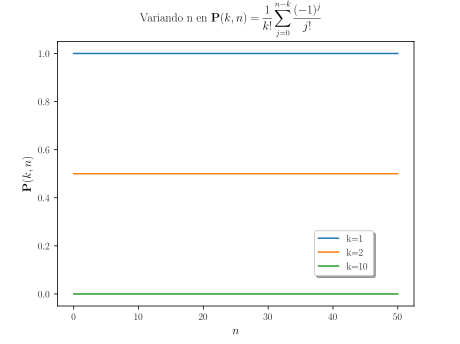
\includegraphics[width=.7\linewidth]{images/graph_nvar.svg}
     %\resizebox{0.7\textwidth}{!}{\input{images/graph_kvar.pgf}}
  \caption{Gráfico variando $n$ y manteniendo $k$ constante}\label{fig:data1}
\end{figure}
\newpage

Entre tanto el gráfico que varia los valores de $k$ y mantiene fijo $n$ (ver \figref{fig:data2}), obtenemos una curva que tiene un punto máximo y luego decae exponencialmente y se mantiene constante en $0$. Esto nos señala que la probabilidad de tener $k$ puntos fijos es máxima sólo cuando $k \in [0,1]$ aproximadamente, o cuando queremos poca cantidad de puntos fijos $(k<5)$ donde, a pesar que no es máxima, la probabilidad es mayor a $0.5$. Mientra que, por el contrario, para $k>5$ la probabilidad tener $k$ puntos fijos se aproxima a 0. El resultado es similar al obtenido en el gráfico anterior, además se obtiene que la probabilidad de que la cantidad de puntos fijos sea igual a $n$ es $P(X=n)=0$ aproximadamente.\\

\begin{figure}[htp]
  \centering
  \includesvg[width=0.65\linewidth]{images/graph_kvar.svg}
     %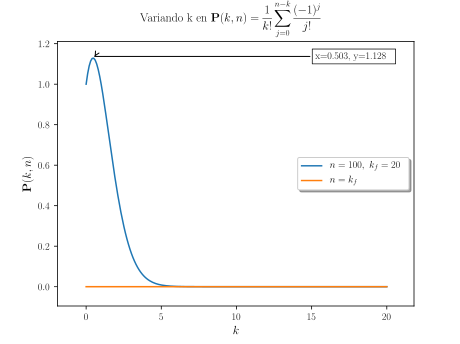
\includegraphics[width=.7\linewidth]{images/graph_kvar.svg}
     %\resizebox{0.7\textwidth}{!}{\input{images/graph_nvar.pgf}}
  \caption{Gráfico variando $k$ y manteniendo $n$ constante}\label{fig:data2}
\end{figure}
\newpage

\begin{tcolorbox}[colback=red!5!white,colframe=red!75!black]
\boxed{\textbf{P2}} Sea $V = \{a,b\}$ un conjunto de nombres de variables, $C = \{1,2\}$ subconjunto de los naturales (Se pueden considerar ambos como conjuntos de símbolos). Se define $\mathcal{EXP}$ como un conjunto de expresiones sobre $\Sigma = {+,*,=,(,)} \cup V \cup C$ como: 
\begin{itemize}
  \item \textbf{Regla Base:} Si $a \in V \cup C$ entonces $a \in \mathcal{EXP}$
  \item \textbf{Regla 2:} Si $a,b \in \mathcal{EXP}$ entonces $(a + b) \in \mathcal{EXP}$
  \item \textbf{Regla 3:} Si $a,b \in \mathcal{EXP}$ entonces $(a * b) \in \mathcal{EXP}$
  \item \textbf{Regla 4:} Si $a,b \in \mathcal{EXP}$ entonces $(a == b) \in \mathcal{EXP}$
\end{itemize}
\end{tcolorbox}

\textbf{Nota: } Para las siguientes preguntas vamos a considerar en ocasiones $\epsilon \in V\cup C$ y $\sigma \in \{+,*,==\} $

\begin{tcolorbox}
\boxed{\textbf{P2.1}} Sea $a_n $ la cantidad de expresiones en $\mathcal{EXP}$ distintas con largo $n$. Entregue una relación de recurrencia para $a_n$ 
\end{tcolorbox}

Para encontrar $a_{n}$ primero nos damos cuenta de cómo se construye cada elemento en $\EXP$. Las reglas bases de $\EXP$ definen strings de largo $\{1,5,6\}$ donde la regla base permite obtener las combinaciones posibles para $\{(a + b), (a * b), (a==b)\}$ que son $\{4^2, 4^2 ,4^2\} $ respectivamente. Luego, cada largo tiene su respectiva combinación, es decir se generan las tuplas de la forma $(n,a_n)$ como $\{ (1,4), (5,4^2 \cdot 2), (6, 4^2) \}$, donde es importante resaltar que dado a que $n=5$ tiene $2$ maneras de obtenerse, entonces se debe multiplicar por 2 el resultado de $a_n $. Entonces, para formar la recurrencia, debemos considerar que para cada $n$ el valor de $a_n $ puede estar en 3 casos:

\begin{itemize}
  \item casos bases: $[n=1 \Rightarrow a_n=4], [n=5 \Rightarrow a_n=4^2 \cdot 2], [n=6 \Rightarrow a_n=4^2]$. Notar que los casos $n<6$, con $n\not\in \{1,5,6\}$ implican $a_n=0$ 
  \item caso $(n>6)$ se divide en tres:
  \begin{itemize}
    \item caso $a_{n-3}$, asumiendo que la expresion es de la forma $(e_1 \{+,*\} e_2)$, en donde anotamos el largo de $e_1$ como $i$, y por tanto el largo de $e_2$ como $n-3-i$. Luego notamos que $e_1$ y $e_2$ poseen largos que pueden ya pudieron ser evaluados, es decir que son obtenidos con $a_{i} $ y $a_{n-3-i}$ respectivamente. Además, tenemos que si $e_1 \neq e_2$ entonces $e_1 {+,*} e_2 \neq e_2 {+,*} e_1$, por lo que la expresión se puede ordenar de 2 formas distintas. Por tanto nos quedaría la expresión:$= (a_{i} + a_{n-3-i})\cdot 2$
    \begin{equation*}
    a_{n-3}= \left\{
    \begin{aligned}
        &0\ \ &si\ \ (i\wedge (n-3-i)) \not\in \{1,5,6\}  \\
        &(a_{i} + a_{n-3-i})\cdot 2 \cdot 2\ \ &si\ \ e_1 \neq e_2\\
        &(a_{i} + a_{n-3-i})\cdot 2 \ \ &si\ \ e_1 = e_2
    \end{aligned}
    \right.    
    \end{equation*}
    \item caso $a_{n-4}$, asumiendo que la expresion es de la forma $(e_3 \{==\} e_4)$, en donde asumimos que $e_3$ tiene largo $j$, y por tanto $e_4 $ tien largo $n-4-j$, obtenemos un resultado similar al anterior:
    \begin{equation*}
    a_{n-4}= \left\{
    \begin{aligned}
        &0\ \ &si\ \ (i\wedge (n-4-i)) \not\in \{1,5,6\}  \\
        &(a_{j} + a_{n-4-j})\cdot 2\ \ &si\ \ e_1 \neq e_2\\
        &(a_{j} + a_{n-4-j}) \ \ &si\ \ e_1 = e_2
    \end{aligned}
    \right.    
    \end{equation*}
  \end{itemize}
\end{itemize}

De esta forma definimos la recursión como:
\begin{equation}
  a_{n} = a_{n-3} + a_{n-4}
\end{equation}

\begin{tcolorbox}
\boxed{\textbf{P2.2}} Programe una función cantidad que reciba como parámetro un natural $n$ y entregue $a_n$ 
\end{tcolorbox}

Para realizar el algoritmo \texttt{cantidad} que calcula $a_n$ se opta por 1 idea de 3 que se complementan. Las ideas son:

\begin{enumerate}
  \item Crear arbol binario con dos llaves, donde la primera llave es el largo del string, y la segunda llave es cuantas maneras distintas puede aparecer una llave con caracteristicas semejantes. Por ejemplo $\{+, *, ==\}$ son nodos $(3,2)$, $(3,2)$ y $(4,1)$ respectivamente (notar que se consideran los parentesis en el conteo), y la misma idea es para los elementos tipo $\epsilon$, pero sin considerar parentésis. El problema con esta idea era la implementación de las funciones para comparar entre arboles, la consideración de parentesis, entre otros.
  \item La segunda opción fue elaborar dos matrices, una que almacenara los largos posibles que cumplan las condiciones de pertenecer a $\mathcal{EXP}$, y otra que almacenara las combinaciones posibles de tener un cierto largo.
\begin{table}[htbp]
  \centering
\begin{minipage}[h]{0.4\linewidth}
\begin{tikzpicture}[thick, 
  level 1/.style={sibling distance=4cm, level distance=3cm},
  level 2/.style={sibling distance=2cm, level distance=3cm}]
\node {    \begin{tabular}{|c|cc|c|}
\cline{2-4}    \rowcolor[rgb]{ .051,  .051,  .051} \multicolumn{1}{c|}{} & \multicolumn{1}{c|}{\cellcolor[rgb]{ 1,  .902,  .6}1} & \cellcolor[rgb]{ 1,  .902,  .6}5 & \cellcolor[rgb]{ 1,  .902,  .6}6 \bigstrut\\
    \hline
    \rowcolor[rgb]{ 1,  .902,  .6} 1     & \multicolumn{1}{c|}{\cellcolor[rgb]{ 1,  1,  1}2} & \cellcolor[rgb]{ 1,  1,  1}6 & \cellcolor[rgb]{ 1,  1,  1}7 \bigstrut\\
    \hline
    \rowcolor[rgb]{ 1,  .902,  .6} 5     & \multicolumn{1}{c|}{\cellcolor[rgb]{ .051,  .051,  .051}} & \cellcolor[rgb]{ 1,  1,  1}10 & \cellcolor[rgb]{ 1,  1,  1}11 \bigstrut\\
\cline{1-1}\cline{3-4}    \rowcolor[rgb]{ 1,  .902,  .6} 6     & \cellcolor[rgb]{ .051,  .051,  .051} & \cellcolor[rgb]{ .051,  .051,  .051} & \cellcolor[rgb]{ 1,  1,  1}12 \bigstrut\\
\cline{1-1}\cline{4-4}    \end{tabular}}
  child {node{    \begin{tabular}{|c|cc|c|}
\cline{2-4}    \rowcolor[rgb]{ .051,  .051,  .051} \multicolumn{1}{c|}{} & \multicolumn{1}{c|}{\cellcolor[rgb]{ 1,  .902,  .6}1} & \cellcolor[rgb]{ 1,  .902,  .6}5 & \cellcolor[rgb]{ 1,  .902,  .6}6 \bigstrut\\
    \hline
    \rowcolor[rgb]{ 1,  .902,  .6} 1     & \multicolumn{1}{c|}{\cellcolor[rgb]{ 1,  1,  1}5} & \cellcolor[rgb]{ .776,  .878,  .706}9 & \cellcolor[rgb]{ .776,  .878,  .706}10 \bigstrut\\
    \hline
    \rowcolor[rgb]{ 1,  .902,  .6} 5     & \multicolumn{1}{c|}{\cellcolor[rgb]{ .051,  .051,  .051}} & \cellcolor[rgb]{ .776,  .878,  .706}13 & \cellcolor[rgb]{ .776,  .878,  .706}14 \bigstrut\\
\cline{1-1}\cline{3-4}    \rowcolor[rgb]{ 1,  .902,  .6} 6     & \cellcolor[rgb]{ .051,  .051,  .051} & \cellcolor[rgb]{ .051,  .051,  .051} & \cellcolor[rgb]{ .776,  .878,  .706}15 \bigstrut\\
\cline{1-1}\cline{4-4}    \end{tabular}}
  }
  child {node {    \begin{tabular}{|c|cc|c|}
\cline{2-4}    \rowcolor[rgb]{ .051,  .051,  .051} \multicolumn{1}{c|}{} & \multicolumn{1}{c|}{\cellcolor[rgb]{ .973,  .796,  .678}1} & \cellcolor[rgb]{ .973,  .796,  .678}5 & \cellcolor[rgb]{ .973,  .796,  .678}6 \bigstrut\\
    \hline
    \rowcolor[rgb]{ .973,  .796,  .678} 1     & \multicolumn{1}{c|}{\cellcolor[rgb]{ 1,  1,  1}6} & \cellcolor[rgb]{ .706,  .776,  .906}10 & \cellcolor[rgb]{ .706,  .776,  .906}11 \bigstrut\\
    \hline
    \rowcolor[rgb]{ .973,  .796,  .678} 5     & \multicolumn{1}{c|}{\cellcolor[rgb]{ .051,  .051,  .051}} & \cellcolor[rgb]{ .706,  .776,  .906}14 & \cellcolor[rgb]{ .706,  .776,  .906}15 \bigstrut\\
\cline{1-1}\cline{3-4}    \rowcolor[rgb]{ .973,  .796,  .678} 6     & \cellcolor[rgb]{ .051,  .051,  .051} & \cellcolor[rgb]{ .051,  .051,  .051} & \cellcolor[rgb]{ .706,  .776,  .906}16 \bigstrut\\
\cline{1-1}\cline{4-4}    \end{tabular}}
  };
\end{tikzpicture}
\captionof{figure}{Matriz de largos bases generadora de matrices elementos (+3, izquierda) o (+4, derecha)}
\label{fig:largost}  
\end{minipage}
\end{table}
En la \textbf{\figref{fig:largost}} se muestra una representación de la matriz con los valores posibles sumando los largos bases, es decir $\{1,5,6\}$. La matriz generada, se divide en dos posibles resultados futuros: cuando el operador es $\{+,*\}$ \textit{(matriz de la izquieda)} entonces a cada elemento de la matriz que no tiene borde amarillo se le suma 3 (pues se suman 3 nuevos carácteres a la expresión, considerando los paréntesis), cuando el operador es $\{==\}$ \textit{(matriz de la derecha)} se le suma 4.

\begin{table}[htbp]
  \centering
\begin{minipage}[h]{0.4\linewidth}
\begin{tikzpicture}[thick, 
  level 1/.style={sibling distance=4cm, level distance=3cm},
  level 2/.style={sibling distance=2cm, level distance=3cm},]
\node {    
    \begin{tabular}{|c|c|c|c|}
    \hline
    \rowcolor[rgb]{ 0,  0,  0}       & \cellcolor[rgb]{ 1,  .902,  .6}4 & \cellcolor[rgb]{ 1,  .902,  .6}32 & \cellcolor[rgb]{ 1,  .902,  .6}16 \bigstrut\\
    \hline
    \rowcolor[rgb]{ 1,  .902,  .6} 4     & \cellcolor[rgb]{ 1,  1,  1}16 & \cellcolor[rgb]{ 1,  1,  1}128 & \cellcolor[rgb]{ 1,  1,  1}64 \bigstrut\\
    \hline
    \rowcolor[rgb]{ 1,  .902,  .6} 32    & \cellcolor[rgb]{ 0,  0,  0} & \cellcolor[rgb]{ 1,  1,  1}1024 & \cellcolor[rgb]{ 1,  1,  1}512 \bigstrut\\
    \hline
    \rowcolor[rgb]{ 1,  .902,  .6} 16    & \cellcolor[rgb]{ 0,  0,  0} & \cellcolor[rgb]{ 0,  0,  0} & \cellcolor[rgb]{ 1,  1,  1}256 \bigstrut\\
    \hline
    \end{tabular}%
}
  child {node{
    \begin{tabular}{|c|c|c|c|}
    \hline
    \rowcolor[rgb]{ 0,  0,  0}       & \cellcolor[rgb]{ 1,  .902,  .6}4 & \cellcolor[rgb]{ 1,  .902,  .6}32 & \cellcolor[rgb]{ 1,  .902,  .6}16 \bigstrut\\
    \hline
    \rowcolor[rgb]{ 1,  .902,  .6} 4     & \cellcolor[rgb]{ 1,  1,  1}32 & \cellcolor[rgb]{ .776,  .878,  .706}256 & \cellcolor[rgb]{ .776,  .878,  .706}128 \bigstrut\\
    \hline
    \rowcolor[rgb]{ 1,  .902,  .6} 32    & \cellcolor[rgb]{ 0,  0,  0} & \cellcolor[rgb]{ .776,  .878,  .706}2048 & \cellcolor[rgb]{ .776,  .878,  .706}1024 \bigstrut\\
    \hline
    \rowcolor[rgb]{ 1,  .902,  .6} 16    & \cellcolor[rgb]{ 0,  0,  0} & \cellcolor[rgb]{ 0,  0,  0} & \cellcolor[rgb]{ .776,  .878,  .706}512 \bigstrut\\
    \hline
    \end{tabular}%
}
  }
  child {node {    
    \begin{tabular}{|c|c|c|c|}
    \hline
    \rowcolor[rgb]{ 0,  0,  0}       & \cellcolor[rgb]{ .973,  .796,  .678}4 & \cellcolor[rgb]{ .973,  .796,  .678}32 & \cellcolor[rgb]{ .973,  .796,  .678}16 \bigstrut\\
    \hline
    \rowcolor[rgb]{ .973,  .796,  .678} 4     & \cellcolor[rgb]{ 1,  1,  1}16 & \cellcolor[rgb]{ .741,  .843,  .933}128 & \cellcolor[rgb]{ .741,  .843,  .933}64 \bigstrut\\
    \hline
    \rowcolor[rgb]{ .973,  .796,  .678} 32    & \cellcolor[rgb]{ 0,  0,  0} & \cellcolor[rgb]{ .741,  .843,  .933}1024 & \cellcolor[rgb]{ .741,  .843,  .933}512 \bigstrut\\
    \hline
    \rowcolor[rgb]{ .973,  .796,  .678} 16    & \cellcolor[rgb]{ 0,  0,  0} & \cellcolor[rgb]{ 0,  0,  0} & \cellcolor[rgb]{ .741,  .843,  .933}256 \bigstrut\\
    \hline
    \end{tabular}%
}
  };
\end{tikzpicture}
\captionof{figure}{matriz de combinaciones posibles}
\label{fig:matcombi}  
\end{minipage}
\end{table}

Mientras que la segunda matriz de combinaciones posibles es como se muestra en \textbf{\figref{fig:matcombi}}, donde \textit{la matriz de la izquierda} representa cuando el operador principal (entiéndase por principal aquel operador que contiene a dos expresiones y no es hijo de otro operador) es $\{+,*\}$ entonces se multiplica por 2 los elementos de la matriz, pues hay dos maneras de generarlo. Para \textit{la matriz de la derecha}, el operador principal es $\{==\}$ por lo que se deja tal cual la matriz, pues hay una forma solamente de formar una expresión así.

Luego, es importante recalcar que el resultado final depende de la posición en la que se ubique la combinación, pues para elementos en la posición $(i,i)$ con $i\in\{1,5,6\}$ no hay forma de conmutar los indices, pues son igual, en cambio para combinaciones en la posición $(i,j)$ tenemos que $(i,j)\neq (j,i)$ pues nos interesa el orden, por tanto hay que multiplicar por 2 estos resultados en el output.

El problema con esta idea era generar ambas matrices, y para valores de $n$ más grades ocupa mucha memoria. Además, en la búsqueda del elemento de la matriz es necesario consultar primero la matriz de largo, y luego consultar la posición del largo en la matriz de combinaciones. Por último, si se necesita agrandar la matriz de largos, también es necesario agrandar la matriz de combinaciones, por lo que se vuelve más engorroso.

\item La solución a los dos problemas anteriores fue ocupar la idea 2 pero uniendo ambas matrices en una, formando tuplas con el largo del string y con el número de combinaciones. En el siguiente ejemplo \textbf{(Ver \figref{fig:tuplas})} la matriz ``padre'' es la que genera a las matrices que tienen los largos de expresiones posibles con su combinaciones respectivas, semejante a la idea anterior, la matriz de la izquierda suma a los elementos de adentro 3, pues representa a una posible \textit{sub expresión} :
\begin{table}[h]
\centering
\begin{minipage}[h]{0.8\linewidth}
\begin{tikzpicture}[thick, 
  level 1/.style={sibling distance=7cm, level distance=3cm}]
\node {    
    \begin{tabular}{|c|c|c|c|}
    \hline
    \rowcolor[rgb]{ 0,  0,  0}       & \cellcolor[rgb]{ 1,  .902,  .6}$\{1,4\}$ & \cellcolor[rgb]{ 1,  .902,  .6}$\{5,32\} $ & \cellcolor[rgb]{ 1,  .902,  .6}$\{6,16\} $\bigstrut\\
    \hline
    \rowcolor[rgb]{ 1,  .902,  .6} $\{1,4\}$ & \cellcolor[rgb]{ 1,  1,  1}$\{2,16\}$ & \cellcolor[rgb]{ 1,  1,  1}$\{6,128\}$ & \cellcolor[rgb]{ 1,  1,  1}$\{7,64\}$ \bigstrut\\
    \hline
    \rowcolor[rgb]{ 1,  .902,  .6} $\{5,32\} $ & \cellcolor[rgb]{ 0,  0,  0} & \cellcolor[rgb]{ 1,  1,  1}$\{10,1024\}$ & \cellcolor[rgb]{ 1,  1,  1}$\{11,512\}$ \bigstrut\\
    \hline
    \rowcolor[rgb]{ 1,  .902,  .6} $\{6,16\} $ & \cellcolor[rgb]{ 0,  0,  0} & \cellcolor[rgb]{ 0,  0,  0} & \cellcolor[rgb]{ 1,  1,  1}$\{12,256\}$ \bigstrut\\
    \hline
    \end{tabular}%
}
  child {node{
    \begin{tabular}{|c|c|c|c|}
    \hline
    \rowcolor[rgb]{ 0,  0,  0}       & \cellcolor[rgb]{ 1,  .902,  .6}$\{1,4\}$ & \cellcolor[rgb]{ 1,  .902,  .6}$\{5,32\} $ & \cellcolor[rgb]{ 1,  .902,  .6}$\{6,16\} $ \bigstrut\\
    \hline
    \rowcolor[rgb]{ 1,  .902,  .6} $\{1,4\}$ & \cellcolor[rgb]{ 1,  1,  1}$\{5,32\}$ & \cellcolor[rgb]{ .776,  .878,  .706}$\{9,256\}$ & \cellcolor[rgb]{ .776,  .878,  .706}$\{10,128\}$ \bigstrut\\
    \hline
    \rowcolor[rgb]{ 1,  .902,  .6} $\{5,32\} $ & \cellcolor[rgb]{ 0,  0,  0} & \cellcolor[rgb]{ .776,  .878,  .706}$\{13,2048\}$ & \cellcolor[rgb]{ .776,  .878,  .706}$\{14,1024\}$ \bigstrut\\
    \hline
    \rowcolor[rgb]{ 1,  .902,  .6} $\{6,16\} $ & \cellcolor[rgb]{ 0,  0,  0} & \cellcolor[rgb]{ 0,  0,  0} & \cellcolor[rgb]{ .776,  .878,  .706}$\{15,512\}$ \bigstrut\\
    \hline
    \end{tabular}%
}
  }
  child {node {    
    \begin{tabular}{|c|c|c|c|}
    \hline
    \rowcolor[rgb]{ 0,  0,  0}       & \cellcolor[rgb]{ 1,  .902,  .6}$\{1,4\}$ & \cellcolor[rgb]{ 1,  .902,  .6}$\{5,32\} $ & \cellcolor[rgb]{ 1,  .902,  .6}$\{6,16\} $\bigstrut\\
    \hline
    \rowcolor[rgb]{ 1,  .902,  .6} $\{1,4\}$ & \cellcolor[rgb]{ 1,  1,  1}$\{6,16\}$ & \cellcolor[rgb]{ .973,  .796,  .678}$\{10,128\}$ & \cellcolor[rgb]{ .973,  .796,  .678}$\{11,64\}$ \bigstrut\\
    \hline
    \rowcolor[rgb]{ 1,  .902,  .6} $\{5,32\} $ & \cellcolor[rgb]{ 0,  0,  0} & \cellcolor[rgb]{ .973,  .796,  .678}$\{14,1024\}$ & \cellcolor[rgb]{ .973,  .796,  .678}$\{15,512\}$ \bigstrut\\
    \hline
    \rowcolor[rgb]{ 1,  .902,  .6} $\{6,16\} $ & \cellcolor[rgb]{ 0,  0,  0} & \cellcolor[rgb]{ 0,  0,  0} & \cellcolor[rgb]{ .973,  .796,  .678}$\{16,256\}$ \bigstrut\\
    \hline
    \end{tabular}%
}
  };
\end{tikzpicture}
\captionof{figure}{Matriz generadora, versión tuplas}
\label{fig:tuplas}   
\end{minipage}
\end{table}

La ventaja de esta idea es que nos genera matrices que son más fáciles de manejar y de expandir, y que al momento de consultar obtenemos dos datos en el mismo instante. Además, se logra apreciar de mejor manera más formas de encontrar combinaciones de un número. Por ejemplo, en la idea anterior existía el problema que al momento de expandir la matriz de combinaciones \textbf{(Ver \figref{fig:matcombi4})} se generaban matrices con un largo mayor al doble de la matriz ``padre'', lo que dificultaba aún más la búsqueda de la combinación correspondiente.

\begin{table}[htbp]
\centering
\begin{minipage}[h]{0.8\linewidth}
\begin{tikzpicture}[thick, 
  level 1/.style={sibling distance=8cm, level distance=4.5cm}]
\node { \begin{tabular}{|c|cc|c|}
\cline{2-4}    \rowcolor[rgb]{ .051,  .051,  .051} \multicolumn{1}{c|}{} & \multicolumn{1}{c|}{\cellcolor[rgb]{ .973,  .796,  .678}1} & \cellcolor[rgb]{ .973,  .796,  .678}5 & \cellcolor[rgb]{ .973,  .796,  .678}6 \bigstrut\\
    \hline
    \rowcolor[rgb]{ .973,  .796,  .678} 1     & \multicolumn{1}{c|}{\cellcolor[rgb]{ 1,  1,  1}6} & \cellcolor[rgb]{ .706,  .776,  .906}10 & \cellcolor[rgb]{ .706,  .776,  .906}11 \bigstrut\\
    \hline
    \rowcolor[rgb]{ .973,  .796,  .678} 5     & \multicolumn{1}{c|}{\cellcolor[rgb]{ .051,  .051,  .051}} & \cellcolor[rgb]{ .706,  .776,  .906}14 & \cellcolor[rgb]{ .706,  .776,  .906}15 \bigstrut\\
\cline{1-1}\cline{3-4}    \rowcolor[rgb]{ .973,  .796,  .678} 6     & \cellcolor[rgb]{ .051,  .051,  .051} & \cellcolor[rgb]{ .051,  .051,  .051} & \cellcolor[rgb]{ .706,  .776,  .906}16 \bigstrut\\
\cline{1-1}\cline{4-4}    \end{tabular}}
child{node {
    \begin{tabular}{|c|rrrrrrr|c|}
\cline{2-9}    \rowcolor[rgb]{ .051,  .051,  .051} \multicolumn{1}{c|}{} & \multicolumn{1}{c|}{\cellcolor[rgb]{ .973,  .796,  .678}1} & \multicolumn{1}{c|}{\cellcolor[rgb]{ .973,  .796,  .678}5} & \multicolumn{1}{c|}{\cellcolor[rgb]{ .973,  .796,  .678}6} & \multicolumn{1}{c|}{\cellcolor[rgb]{ .973,  .796,  .678}9} & \multicolumn{1}{c|}{\cellcolor[rgb]{ .973,  .796,  .678}10} & \multicolumn{1}{c|}{\cellcolor[rgb]{ .973,  .796,  .678}13} & \multicolumn{1}{c|}{\cellcolor[rgb]{ .973,  .796,  .678}14} & \cellcolor[rgb]{ .973,  .796,  .678}15 \bigstrut\\
    \hline
    \rowcolor[rgb]{ .973,  .796,  .678} 1     & \multicolumn{1}{c|}{\cellcolor[rgb]{ 1,  1,  1}6} & \multicolumn{1}{c|}{\cellcolor[rgb]{ 1,  1,  1}10} & \multicolumn{1}{c|}{\cellcolor[rgb]{ 1,  1,  1}11} & \multicolumn{1}{c|}{\cellcolor[rgb]{ .706,  .776,  .906}14} & \multicolumn{1}{c|}{\cellcolor[rgb]{ .706,  .776,  .906}15} & \multicolumn{1}{c|}{\cellcolor[rgb]{ .706,  .776,  .906}18} & \multicolumn{1}{c|}{\cellcolor[rgb]{ .706,  .776,  .906}19} & \cellcolor[rgb]{ .706,  .776,  .906}20 \bigstrut\\
    \hline
    \rowcolor[rgb]{ .973,  .796,  .678} 5     & \multicolumn{1}{c|}{\cellcolor[rgb]{ .051,  .051,  .051}} & \multicolumn{1}{c|}{\cellcolor[rgb]{ 1,  1,  1}14} & \multicolumn{1}{c|}{\cellcolor[rgb]{ 1,  1,  1}15} & \multicolumn{1}{c|}{\cellcolor[rgb]{ .706,  .776,  .906}18} & \multicolumn{1}{c|}{\cellcolor[rgb]{ .706,  .776,  .906}19} & \multicolumn{1}{c|}{\cellcolor[rgb]{ .706,  .776,  .906}22} & \multicolumn{1}{c|}{\cellcolor[rgb]{ .706,  .776,  .906}23} & \cellcolor[rgb]{ .706,  .776,  .906}24 \bigstrut\\
\cline{1-1}\cline{3-9}    \rowcolor[rgb]{ .973,  .796,  .678} 6     & \cellcolor[rgb]{ .051,  .051,  .051} & \multicolumn{1}{c|}{\cellcolor[rgb]{ .051,  .051,  .051}} & \multicolumn{1}{c|}{\cellcolor[rgb]{ 1,  1,  1}16} & \multicolumn{1}{c|}{\cellcolor[rgb]{ .706,  .776,  .906}19} & \multicolumn{1}{c|}{\cellcolor[rgb]{ .706,  .776,  .906}20} & \multicolumn{1}{c|}{\cellcolor[rgb]{ .706,  .776,  .906}23} & \multicolumn{1}{c|}{\cellcolor[rgb]{ .706,  .776,  .906}24} & \cellcolor[rgb]{ .706,  .776,  .906}25 \bigstrut\\
\cline{1-1}\cline{4-9}    \rowcolor[rgb]{ .973,  .796,  .678} 9     & \cellcolor[rgb]{ .051,  .051,  .051} & \cellcolor[rgb]{ .051,  .051,  .051} & \multicolumn{1}{r|}{\cellcolor[rgb]{ .051,  .051,  .051}} & \multicolumn{1}{c|}{\cellcolor[rgb]{ .706,  .776,  .906}22} & \multicolumn{1}{c|}{\cellcolor[rgb]{ .706,  .776,  .906}23} & \multicolumn{1}{c|}{\cellcolor[rgb]{ .706,  .776,  .906}26} & \multicolumn{1}{c|}{\cellcolor[rgb]{ .706,  .776,  .906}27} & \cellcolor[rgb]{ .706,  .776,  .906}28 \bigstrut\\
\cline{1-1}\cline{5-9}    \rowcolor[rgb]{ .973,  .796,  .678} 10    & \cellcolor[rgb]{ .051,  .051,  .051} & \cellcolor[rgb]{ .051,  .051,  .051} & \cellcolor[rgb]{ .051,  .051,  .051} & \multicolumn{1}{r|}{\cellcolor[rgb]{ .051,  .051,  .051}} & \multicolumn{1}{c|}{\cellcolor[rgb]{ .706,  .776,  .906}24} & \multicolumn{1}{c|}{\cellcolor[rgb]{ .706,  .776,  .906}27} & \multicolumn{1}{c|}{\cellcolor[rgb]{ .706,  .776,  .906}28} & \cellcolor[rgb]{ .706,  .776,  .906}29 \bigstrut\\
\cline{1-1}\cline{6-9}    \rowcolor[rgb]{ .973,  .796,  .678} 13    & \cellcolor[rgb]{ .051,  .051,  .051} & \cellcolor[rgb]{ .051,  .051,  .051} & \cellcolor[rgb]{ .051,  .051,  .051} & \cellcolor[rgb]{ .051,  .051,  .051} & \multicolumn{1}{r|}{\cellcolor[rgb]{ .051,  .051,  .051}} & \multicolumn{1}{c|}{\cellcolor[rgb]{ .706,  .776,  .906}30} & \multicolumn{1}{c|}{\cellcolor[rgb]{ .706,  .776,  .906}31} & \cellcolor[rgb]{ .706,  .776,  .906}32 \bigstrut\\
\cline{1-1}\cline{7-9}    \rowcolor[rgb]{ .973,  .796,  .678} 14    & \cellcolor[rgb]{ .051,  .051,  .051} & \cellcolor[rgb]{ .051,  .051,  .051} & \cellcolor[rgb]{ .051,  .051,  .051} & \cellcolor[rgb]{ .051,  .051,  .051} & \cellcolor[rgb]{ .051,  .051,  .051} & \multicolumn{1}{r|}{\cellcolor[rgb]{ .051,  .051,  .051}} & \multicolumn{1}{c|}{\cellcolor[rgb]{ .706,  .776,  .906}32} & \cellcolor[rgb]{ .706,  .776,  .906}33 \bigstrut\\
\cline{1-1}\cline{8-9}    \rowcolor[rgb]{ .973,  .796,  .678} 15    & \cellcolor[rgb]{ .051,  .051,  .051} & \cellcolor[rgb]{ .051,  .051,  .051} & \cellcolor[rgb]{ .051,  .051,  .051} & \cellcolor[rgb]{ .051,  .051,  .051} & \cellcolor[rgb]{ .051,  .051,  .051} & \cellcolor[rgb]{ .051,  .051,  .051} & \cellcolor[rgb]{ .051,  .051,  .051} & \cellcolor[rgb]{ .706,  .776,  .906}34 \bigstrut\\
\cline{1-1}\cline{9-9}    \end{tabular}%
}
}
child{
  node{
    \begin{tabular}{|c|rrrrrrr|c|}
\cline{2-9}    \rowcolor[rgb]{ .051,  .051,  .051} \multicolumn{1}{c|}{} & \multicolumn{1}{c|}{\cellcolor[rgb]{ .973,  .796,  .678}1} & \multicolumn{1}{c|}{\cellcolor[rgb]{ .973,  .796,  .678}5} & \multicolumn{1}{c|}{\cellcolor[rgb]{ .973,  .796,  .678}6} & \multicolumn{1}{c|}{\cellcolor[rgb]{ .973,  .796,  .678}10} & \multicolumn{1}{c|}{\cellcolor[rgb]{ .973,  .796,  .678}11} & \multicolumn{1}{c|}{\cellcolor[rgb]{ .973,  .796,  .678}14} & \multicolumn{1}{c|}{\cellcolor[rgb]{ .973,  .796,  .678}15} & \cellcolor[rgb]{ .973,  .796,  .678}16 \bigstrut\\
    \hline
    \rowcolor[rgb]{ .973,  .796,  .678} 1     & \multicolumn{1}{c|}{\cellcolor[rgb]{ 1,  1,  1}6} & \multicolumn{1}{c|}{\cellcolor[rgb]{ 1,  1,  1}10} & \multicolumn{1}{c|}{\cellcolor[rgb]{ 1,  1,  1}11} & \multicolumn{1}{c|}{\cellcolor[rgb]{ .706,  .776,  .906}15} & \multicolumn{1}{c|}{\cellcolor[rgb]{ .706,  .776,  .906}16} & \multicolumn{1}{c|}{\cellcolor[rgb]{ .706,  .776,  .906}19} & \multicolumn{1}{c|}{\cellcolor[rgb]{ .706,  .776,  .906}20} & \cellcolor[rgb]{ .706,  .776,  .906}21 \bigstrut\\
    \hline
    \rowcolor[rgb]{ .973,  .796,  .678} 5     & \multicolumn{1}{c|}{\cellcolor[rgb]{ .051,  .051,  .051}} & \multicolumn{1}{c|}{\cellcolor[rgb]{ 1,  1,  1}14} & \multicolumn{1}{c|}{\cellcolor[rgb]{ 1,  1,  1}15} & \multicolumn{1}{c|}{\cellcolor[rgb]{ .706,  .776,  .906}19} & \multicolumn{1}{c|}{\cellcolor[rgb]{ .706,  .776,  .906}20} & \multicolumn{1}{c|}{\cellcolor[rgb]{ .706,  .776,  .906}23} & \multicolumn{1}{c|}{\cellcolor[rgb]{ .706,  .776,  .906}24} & \cellcolor[rgb]{ .706,  .776,  .906}25 \bigstrut\\
\cline{1-1}\cline{3-9}    \rowcolor[rgb]{ .973,  .796,  .678} 6     & \cellcolor[rgb]{ .051,  .051,  .051} & \multicolumn{1}{c|}{\cellcolor[rgb]{ .051,  .051,  .051}} & \multicolumn{1}{c|}{\cellcolor[rgb]{ 1,  1,  1}16} & \multicolumn{1}{c|}{\cellcolor[rgb]{ .706,  .776,  .906}20} & \multicolumn{1}{c|}{\cellcolor[rgb]{ .706,  .776,  .906}21} & \multicolumn{1}{c|}{\cellcolor[rgb]{ .706,  .776,  .906}24} & \multicolumn{1}{c|}{\cellcolor[rgb]{ .706,  .776,  .906}25} & \cellcolor[rgb]{ .706,  .776,  .906}26 \bigstrut\\
\cline{1-1}\cline{4-9}    \rowcolor[rgb]{ .973,  .796,  .678} 10    & \cellcolor[rgb]{ .051,  .051,  .051} & \cellcolor[rgb]{ .051,  .051,  .051} & \multicolumn{1}{r|}{\cellcolor[rgb]{ .051,  .051,  .051}} & \multicolumn{1}{c|}{\cellcolor[rgb]{ .706,  .776,  .906}24} & \multicolumn{1}{c|}{\cellcolor[rgb]{ .706,  .776,  .906}25} & \multicolumn{1}{c|}{\cellcolor[rgb]{ .706,  .776,  .906}28} & \multicolumn{1}{c|}{\cellcolor[rgb]{ .706,  .776,  .906}29} & \cellcolor[rgb]{ .706,  .776,  .906}30 \bigstrut\\
\cline{1-1}\cline{5-9}    \rowcolor[rgb]{ .973,  .796,  .678} 11    & \cellcolor[rgb]{ .051,  .051,  .051} & \cellcolor[rgb]{ .051,  .051,  .051} & \cellcolor[rgb]{ .051,  .051,  .051} & \multicolumn{1}{r|}{\cellcolor[rgb]{ .051,  .051,  .051}} & \multicolumn{1}{c|}{\cellcolor[rgb]{ .706,  .776,  .906}26} & \multicolumn{1}{c|}{\cellcolor[rgb]{ .706,  .776,  .906}29} & \multicolumn{1}{c|}{\cellcolor[rgb]{ .706,  .776,  .906}30} & \cellcolor[rgb]{ .706,  .776,  .906}31 \bigstrut\\
\cline{1-1}\cline{6-9}    \rowcolor[rgb]{ .973,  .796,  .678} 14    & \cellcolor[rgb]{ .051,  .051,  .051} & \cellcolor[rgb]{ .051,  .051,  .051} & \cellcolor[rgb]{ .051,  .051,  .051} & \cellcolor[rgb]{ .051,  .051,  .051} & \multicolumn{1}{r|}{\cellcolor[rgb]{ .051,  .051,  .051}} & \multicolumn{1}{c|}{\cellcolor[rgb]{ .706,  .776,  .906}32} & \multicolumn{1}{c|}{\cellcolor[rgb]{ .706,  .776,  .906}33} & \cellcolor[rgb]{ .706,  .776,  .906}34 \bigstrut\\
\cline{1-1}\cline{7-9}    \rowcolor[rgb]{ .973,  .796,  .678} 15    & \cellcolor[rgb]{ .051,  .051,  .051} & \cellcolor[rgb]{ .051,  .051,  .051} & \cellcolor[rgb]{ .051,  .051,  .051} & \cellcolor[rgb]{ .051,  .051,  .051} & \cellcolor[rgb]{ .051,  .051,  .051} & \multicolumn{1}{r|}{\cellcolor[rgb]{ .051,  .051,  .051}} & \multicolumn{1}{c|}{\cellcolor[rgb]{ .706,  .776,  .906}34} & \cellcolor[rgb]{ .706,  .776,  .906}35 \bigstrut\\
\cline{1-1}\cline{8-9}    \rowcolor[rgb]{ .973,  .796,  .678} 16    & \cellcolor[rgb]{ .051,  .051,  .051} & \cellcolor[rgb]{ .051,  .051,  .051} & \cellcolor[rgb]{ .051,  .051,  .051} & \cellcolor[rgb]{ .051,  .051,  .051} & \cellcolor[rgb]{ .051,  .051,  .051} & \cellcolor[rgb]{ .051,  .051,  .051} & \cellcolor[rgb]{ .051,  .051,  .051} & \cellcolor[rgb]{ .706,  .776,  .906}36 \bigstrut\\
\cline{1-1}\cline{9-9}    \end{tabular}%
  }
};
\end{tikzpicture}
\captionof{figure}{Matrices de combinaciones posible para expresiones con signo ``$==$''}
\label{fig:matcombi4}
\end{minipage}
\end{table}

Con la idea de generar las matrices con tuplas se elimina esta dificultad y sólo basta con buscar el largo del elemento en la matriz, obtener la combinación con la cual se obtiene ese largo (tiempo constante, pues es consultar el otro elemento de la tupla) e ir acumulando el resultado junto con todos los largos posibles, con sus respectivas combinaciones. 
\end{enumerate}

De esta manera, con la última opción es posible encontrar $a_n$ para cada $n$ ingresado, y el algoritmo logra ser recursivo, pues en los casos distintos a los casos bases, es suficiente buscar en la matriz de tuplas, para los valores de $n-3$ (asumiendo que el nodo puede ser $\{+,*\}$) o $n-4$ (asumiendo que el nodo puede ser $\{==\}$), y sumar ambos resultados. En caso de no estar en la matriz por ser mayor a los elementos que están dentro, entonces la matriz se debe agrandar hasta que el elemento que buscamos sea menor al mayor elemento de la matriz (\texttt{mat[m-1][m-1]}, con \texttt{m: largo de la matriz}). 

Las matrices generadas además tienen la ventaja de estar ordenadas de menor a mayor por cada fila, por lo que el algoritmo de búsqueda se puede manejar más fácil. En la implementación realizada en \texttt{cantidad} se realiza el siguiente algoritmo de búsqueda \textbf{(Ver Código \ref{code:search})}, donde \texttt{mat} es la matriz generada por las combinaciones de los distintos largos \textbf{(revisar \figref{fig:tuplas})}, más el factor \texttt{pr} (3 o 4) según la busqueda que se esté realizando (asumiendo que la expresión tiene un operador principal $\{+,*\}$ entonces $pr=3$, si no entonces tiene oper. ppal. $\{==\}$ y $pr=4$); \texttt{x} es $n-3$ o $n-4$, dependiendo de cual buscamos y $col$ representa la columna donde debemos empezar a buscar (columnas pintadas en \figref{fig:tuplas}):

\begin{code}
\captionof{listing}{Búsqueda en matriz}
\label{code:search}
\begin{minted}[bgcolor=bg,frame=lines,framesep=2mm]{python}
def search(mat, x, pr,col):
  n= len(mat[0]) - 1
  i = 0 
  j = n
  arr=[] 
  while ( i <= n and j >= col ): # se comienza en el punto (col,n-1)
    v = mat[i][j]
    if (v[0] == x):
      if pr==3: v[1]*=2
      arr.append(v)
    if (v[0] > x ): j -= 1 
    else:  # if v[0] < x
      i += 1
  return arr
\end{minted}
\end{code}

Finalmente, las otras funciones realizadas para complementar a la función \texttt{cantidad} serán explicadas brevemente pues repiten el procedimiento ya explicado anteriormente:
\begin{itemize}
  \item \texttt{triSup(casos\_bases)}: Recibe una lista ($\mathcal{L} $) que representa la columna en amarillo en \textbf{\figref{fig:tuplas}} y genera una matriz triangular superior $\mathcal{M} $ con tuplas, donde cada tupla $(i,j) \in \mathcal{M} $ representa a $(f_1 + c_1, f_2 * c_2)_(i,j)$, con $(f_1,f_2)_i \in \mathcal{L}$, y $(c_1,c_2)_j \in \mathcal{L}$ de la lista transpuesta.
  \item \texttt{agrandar(matriz, paramétro, columna)}: Matriz representa la matriz que se quiere agrandar, parametro es (3 o 4) dependiendo si se quiere sumar 3 o 4 a los nuevos elementos bases de la futura matriz generadora, y columna representa desde cuál columna es necesario agregar elementos.
  \item \texttt{supMat(matriz, casos\_bases, columna)}: combina los procesos de las os funciones anteriores, retornando la matriz y la lista de \texttt{casos\_bases} agrandados.
  \item \texttt{ctd(n,parametro)}: Realiza el trabajo de cantidad, pero dependiendo del parametro (3 o 4). Con 3 asumimos que la expresión se puede formar con el simbolo ``+,*'', con 4 asumimos que se puede formar con ``==''.
  \item \texttt{cantidad(n)}: Ocupa \texttt{ctd(n,3)} y \texttt{ctd(n,4)} y retorna la suma de ambos, resolviendo la recursión.
\end{itemize}

\textbf{Comentario: } En las pruebas que se realizó al programa sólo es posible llegar a resultados correctos hasta $n=20$. Esto es debido a una mala generalización del problema, eliminando, al agrandar la matriz, elementos que igual hay que sumar al resultado final. El resultado correcto se obtiene eliminando los sectores que se revisaron, y considerando el sector que no se ha revisado. 

\newpage

\begin{tcolorbox}
\boxed{\textbf{P2.3}} Programe una función \texttt{esExp} que reciba como parámetro un string y entregue verdadero si pertenece a $\mathcal{EXP}$ o falso si no.
\end{tcolorbox}

Dado el formato del string, ocupamos el concepto de árbol cartesiano para almacenar los valores de las posiciones. La idea es ir almacenando las operaciones $(+,*, ==)$ en nodos, y las hojas van a ser expresiones basicas, es decir $\{a,b,1,2\}$. La construcción del árbol sigue la siguiente secuencia:

\newdimen\arrowsize
\pgfarrowsdeclare{arcs'}{arcs'}{...}
{
\arrowsize=0.2pt
\advance\arrowsize by .5\pgflinewidth
\pgfsetdash{}{0pt} % do not dash
\pgfsetroundjoin % fix join
\pgfsetroundcap % fix cap
\pgfpathmoveto{\pgfpoint{-4\arrowsize}{4\arrowsize}}
\pgfpatharc{180}{270}{4\arrowsize}
\pgfpatharc{90}{180}{4\arrowsize}
\pgfusepathqstroke
}
\begin{table}[H]
\centering
\begin{minipage}[b]{0.2\linewidth}
\begin{tabular}{|l|}
    \hline
    input \\
    \hline\hline
    ((a*b)+(1==2)) \\
    \hline
    \end{tabular}%
\end{minipage}
\hspace{0.3cm} % Cambiar este espacio
\begin{minipage}[h]{0.05\linewidth}       %%%Aca comienza la flecha
\begin{tikzpicture}
\draw[->,line width=1pt] (-1,0) -- (0,0);
\end{tikzpicture}
\end{minipage}                  %%%Aca termina
\hspace{0.5cm} %Espacio
\begin{minipage}[h]{0.1\linewidth}
\begin{tikzpicture}
\node {+}
  child {node {(a+b)}}
  child {node {(1==2)}};
\end{tikzpicture}
\end{minipage}
\hspace{0.5cm} % Cambiar este espacio
\begin{minipage}[h]{0.05\linewidth}       %%%Aca comienza la flecha
\begin{tikzpicture}
\draw[->,line width=1pt] (-1,0) -- (0,0);
\end{tikzpicture}
\end{minipage}                  %%%Aca termina
\hspace{0.3cm} %Espacio
\begin{minipage}[h]{0.3\linewidth}
\begin{tikzpicture}[thick, 
  level 1/.style={sibling distance=4cm, level distance=1.5cm},
  level 2/.style={sibling distance=2cm, level distance=1.5cm},]
\node {+}
  child {node{*}
    child {node{a}}
    child {node{b}}}
  child {node {==}
    child{node{1}}
    child{node{2}}
    };
\end{tikzpicture}
\end{minipage}
\end{table}

Notar que lo unico necesario para formar el árbol es detectar las operaciones $(+,*,==)$ en la expresión, pero gracias a la permanencia de los paréntesis esto se traduce a detectar en qué nivel estamos y cuál es la operación principal, es decir, aquella que es nodo padre de las otras dos expresiones. En el ejemplo anterior podemos detectar que primero es $+$, y luego $*$ y $==$ para las otras dos expresiones.\\

De esta manera, nuestros casos bases son cuando:

\begin{itemize}
  \item Expresiones de largo igual 1, es decir $\epsilon \in V\cup C$
  \item Expresiones con $|s|>=5$ con $|s|:$ largo del string, donde las hojas deben ser $\epsilon \in V\cup C$ y los nodos deben ser $\{+,*,==\} $
\end{itemize}

Para generar la recurrencia es necesario observar los 3 subcasos del segundo punto:

\begin{table}[h!]
\centering
\begin{minipage}[h]{0.1\linewidth}
\begin{tikzpicture}
\tikzstyle{suba}= [draw=gray!70, regular polygon, regular polygon sides=3 ]
\node {+}
  child {node[suba] {A}}
  child {node {$\epsilon$}};
\end{tikzpicture}
\end{minipage}
\hspace{0.5cm} % Cambiar este espacio
\begin{minipage}[h]{0.05\linewidth}       %%%Aca comienza la flecha
\begin{tikzpicture}
\draw[->,line width=1pt] (-1,0) -- (0,0);
\end{tikzpicture}
\end{minipage}                  %%%Aca termina
\hspace{1cm} %Espacio
\begin{minipage}[h]{0.11\linewidth}
\begin{tikzpicture}
\tikzstyle{suba}= [draw=gray!70, regular polygon, regular polygon sides=3]
\node {+}
  child {node {$\epsilon$}}
  child {node[suba] {B}};
\end{tikzpicture}
\end{minipage}
\hspace{0.5cm} % Cambiar este espacio
\begin{minipage}[h]{0.05\linewidth}       %%%Aca comienza la flecha
\begin{tikzpicture}
\draw[->,line width=1pt] (-1,0) -- (0,0);
\end{tikzpicture}
\end{minipage}                  %%%Aca termina
\hspace{0.3cm} %Espacio
\begin{minipage}[h]{0.11\linewidth}
\begin{tikzpicture}[thick]
\tikzstyle{suba}= [draw=gray!70, regular polygon, regular polygon sides=3]
\node {+}
  child {node[suba] {A}}
  child {node[suba] {B}};
\end{tikzpicture}
\end{minipage}
\end{table}

Las ilustraciones anteriores representan las siguientes formas de expresiones, $(\textrm{Tree} \{+,*,==\} \epsilon)$, $(\epsilon \{+,*,==\} \textrm{Tree})$, $(\textrm{TreeA} \{+,*,==\} \textrm{TreeB})$, respectivamente. 

Para resolver el problema junto con los casos bases y los subcasos seguimos los siguientes pasos:

\begin{enumerate}
  \item Crear la estructura \texttt{Tree}.
  \item Crear las funciones \texttt{enNum, enOp} que nos devuelven \textcolor{red}{\texttt{True}} si la expresión está en $V\cup C$ o en $\{+,*,==\}$ respectivamente.
  \item Como se explicó anteriormente, para $|s|>=5$ se cumple que los nodos son operadores y las hojas símbolos, por lo que para comprobar si el árbol genera una expresion que pertenezca a $\mathcal{EXP}$ creamos la función \texttt{isTree} que nos devuelve \textcolor{red}{\texttt{True}} si cumple pertenecer al conjunto. El caso base es que el nodo sea algún $\epsilon$, si no,  es un operador y cada sub árbol debe cumplir las condiciones ya mencionadas. Si no es ninguna de las anteriores entonces la expresión está mal escrita, devuelve \textcolor{red}{\texttt{False}}.
  \item Se crea la función \texttt{Constructor} que dado un string nos devuelve un árbol cartesiano que representa al string entregado. Aquí se implementan los casos bases mencionados anteriormente. Los subcasos los resolvemos con la ayuda de los parentesis. 
  \begin{itemize}
     \item En el subcaso del nodo con dos subarboles y el nodo con un caracter a la derecha y un subárbol a la izquierda iniciamos un contador que suma 1 según la cantidad de parentesis abiertos y resta 1 según la cantidad de parentesis cerrados desde el indice 1. Si el contador es 0 entonces el siguiente caracter es el ``operador padre'' y creamos un nodo padre con sus dos hijos, el substring de la izquierda y el substring de la derecha.
     \item En el subcaso del nodo con un caracter a la izquierda y un subarbol a la derecha no podemos iniciar de inmediato el contador de parentesis, pues un caracter $\epsilon$ no lleva. La solución es agregar una nueva condición, y considerar que en este caso el siguiente string será el nodo padre, pues es un operador
   \end{itemize} 
  \item Finalmente se crea la función \texttt{esExp} el cual construye el árbol dado un string, y evaluamos si es árbol cartesiano de $\mathcal{EXP}$ con \texttt{isTree}
\end{enumerate}

\textbf{Nota:} Se asume que se entrega un string sin espacios.

\begin{tcolorbox}
\boxed{\textbf{P2.4}} Entregue un archivo \texttt{expresiones.\{py,java,cpp\}} que reciba por entrada estándar un string $s$ e imprima 2 enteros $a,b$ donde $a$ es booleano que representa si $s \in \mathcal{EXP}$ y $b$ es $a_{|s|}$
\end{tcolorbox}


\end{document}



\begin{table}[h]
\centering
\begin{minipage}[h]{0.8\linewidth}
\begin{tikzpicture}[thick, 
  level 1/.style={sibling distance=8cm, level distance=4.5cm}]
\node {\begin{tabular}{|c|cc|c|}
\cline{2-4}    \rowcolor[rgb]{ .051,  .051,  .051} \multicolumn{1}{c|}{} & \multicolumn{1}{c|}{\cellcolor[rgb]{ 1,  .902,  .6}1} & \cellcolor[rgb]{ 1,  .902,  .6}5 & \cellcolor[rgb]{ 1,  .902,  .6}6 \bigstrut\\
    \hline
    \rowcolor[rgb]{ 1,  .902,  .6} 1     & \multicolumn{1}{c|}{\cellcolor[rgb]{ 1,  1,  1}5} & \cellcolor[rgb]{ .776,  .878,  .706}9 & \cellcolor[rgb]{ .776,  .878,  .706}10 \bigstrut\\
    \hline
    \rowcolor[rgb]{ 1,  .902,  .6} 5     & \multicolumn{1}{c|}{\cellcolor[rgb]{ .051,  .051,  .051}} & \cellcolor[rgb]{ .776,  .878,  .706}13 & \cellcolor[rgb]{ .776,  .878,  .706}14 \bigstrut\\
\cline{1-1}\cline{3-4}    \rowcolor[rgb]{ 1,  .902,  .6} 6     & \cellcolor[rgb]{ .051,  .051,  .051} & \cellcolor[rgb]{ .051,  .051,  .051} & \cellcolor[rgb]{ .776,  .878,  .706}15 \bigstrut\\
\cline{1-1}\cline{4-4}    \end{tabular}
}
child{node {
    \begin{tabular}{|c|rrrrrrr|c|}
\cline{2-9}    \rowcolor[rgb]{ .051,  .051,  .051} \multicolumn{1}{c|}{} & \multicolumn{1}{c|}{\cellcolor[rgb]{ 1,  .902,  .6}1} & \multicolumn{1}{c|}{\cellcolor[rgb]{ 1,  .902,  .6}5} & \multicolumn{1}{c|}{\cellcolor[rgb]{ 1,  .902,  .6}6} & \multicolumn{1}{c|}{\cellcolor[rgb]{ 1,  .902,  .6}9} & \multicolumn{1}{c|}{\cellcolor[rgb]{ 1,  .902,  .6}10} & \multicolumn{1}{c|}{\cellcolor[rgb]{ 1,  .902,  .6}13} & \multicolumn{1}{c|}{\cellcolor[rgb]{ 1,  .902,  .6}14} & \cellcolor[rgb]{ 1,  .902,  .6}15 \bigstrut\\
    \hline
    \rowcolor[rgb]{ 1,  .902,  .6} 1     & \multicolumn{1}{c|}{\cellcolor[rgb]{ 1,  1,  1}5} & \multicolumn{1}{c|}{\cellcolor[rgb]{ 1,  1,  1}9} & \multicolumn{1}{c|}{\cellcolor[rgb]{ 1,  1,  1}10} & \multicolumn{1}{c|}{\cellcolor[rgb]{ .776,  .878,  .706}13} & \multicolumn{1}{c|}{\cellcolor[rgb]{ .776,  .878,  .706}14} & \multicolumn{1}{c|}{\cellcolor[rgb]{ .776,  .878,  .706}17} & \multicolumn{1}{c|}{\cellcolor[rgb]{ .776,  .878,  .706}18} & \cellcolor[rgb]{ .776,  .878,  .706}19 \bigstrut\\
    \hline
    \rowcolor[rgb]{ 1,  .902,  .6} 5     & \multicolumn{1}{c|}{\cellcolor[rgb]{ .051,  .051,  .051}} & \multicolumn{1}{c|}{\cellcolor[rgb]{ 1,  1,  1}13} & \multicolumn{1}{c|}{\cellcolor[rgb]{ 1,  1,  1}14} & \multicolumn{1}{c|}{\cellcolor[rgb]{ .776,  .878,  .706}17} & \multicolumn{1}{c|}{\cellcolor[rgb]{ .776,  .878,  .706}18} & \multicolumn{1}{c|}{\cellcolor[rgb]{ .776,  .878,  .706}21} & \multicolumn{1}{c|}{\cellcolor[rgb]{ .776,  .878,  .706}22} & \cellcolor[rgb]{ .776,  .878,  .706}23 \bigstrut\\
\cline{1-1}\cline{3-9}    \rowcolor[rgb]{ 1,  .902,  .6} 6     & \cellcolor[rgb]{ .051,  .051,  .051} & \multicolumn{1}{c|}{\cellcolor[rgb]{ .051,  .051,  .051}} & \multicolumn{1}{c|}{\cellcolor[rgb]{ 1,  1,  1}15} & \multicolumn{1}{c|}{\cellcolor[rgb]{ .776,  .878,  .706}18} & \multicolumn{1}{c|}{\cellcolor[rgb]{ .776,  .878,  .706}19} & \multicolumn{1}{c|}{\cellcolor[rgb]{ .776,  .878,  .706}22} & \multicolumn{1}{c|}{\cellcolor[rgb]{ .776,  .878,  .706}23} & \cellcolor[rgb]{ .776,  .878,  .706}24 \bigstrut\\
\cline{1-1}\cline{4-9}    \rowcolor[rgb]{ 1,  .902,  .6} 9     & \cellcolor[rgb]{ .051,  .051,  .051} & \cellcolor[rgb]{ .051,  .051,  .051} & \multicolumn{1}{r|}{\cellcolor[rgb]{ .051,  .051,  .051}} & \multicolumn{1}{c|}{\cellcolor[rgb]{ .776,  .878,  .706}21} & \multicolumn{1}{c|}{\cellcolor[rgb]{ .776,  .878,  .706}22} & \multicolumn{1}{c|}{\cellcolor[rgb]{ .776,  .878,  .706}25} & \multicolumn{1}{c|}{\cellcolor[rgb]{ .776,  .878,  .706}26} & \cellcolor[rgb]{ .776,  .878,  .706}27 \bigstrut\\
\cline{1-1}\cline{5-9}    \rowcolor[rgb]{ 1,  .902,  .6} 10    & \cellcolor[rgb]{ .051,  .051,  .051} & \cellcolor[rgb]{ .051,  .051,  .051} & \cellcolor[rgb]{ .051,  .051,  .051} & \multicolumn{1}{r|}{\cellcolor[rgb]{ .051,  .051,  .051}} & \multicolumn{1}{c|}{\cellcolor[rgb]{ .776,  .878,  .706}23} & \multicolumn{1}{c|}{\cellcolor[rgb]{ .776,  .878,  .706}26} & \multicolumn{1}{c|}{\cellcolor[rgb]{ .776,  .878,  .706}27} & \cellcolor[rgb]{ .776,  .878,  .706}28 \bigstrut\\
\cline{1-1}\cline{6-9}    \rowcolor[rgb]{ 1,  .902,  .6} 13    & \cellcolor[rgb]{ .051,  .051,  .051} & \cellcolor[rgb]{ .051,  .051,  .051} & \cellcolor[rgb]{ .051,  .051,  .051} & \cellcolor[rgb]{ .051,  .051,  .051} & \multicolumn{1}{r|}{\cellcolor[rgb]{ .051,  .051,  .051}} & \multicolumn{1}{c|}{\cellcolor[rgb]{ .776,  .878,  .706}29} & \multicolumn{1}{c|}{\cellcolor[rgb]{ .776,  .878,  .706}30} & \cellcolor[rgb]{ .776,  .878,  .706}31 \bigstrut\\
\cline{1-1}\cline{7-9}    \rowcolor[rgb]{ 1,  .902,  .6} 14    & \cellcolor[rgb]{ .051,  .051,  .051} & \cellcolor[rgb]{ .051,  .051,  .051} & \cellcolor[rgb]{ .051,  .051,  .051} & \cellcolor[rgb]{ .051,  .051,  .051} & \cellcolor[rgb]{ .051,  .051,  .051} & \multicolumn{1}{r|}{\cellcolor[rgb]{ .051,  .051,  .051}} & \multicolumn{1}{c|}{\cellcolor[rgb]{ .776,  .878,  .706}31} & \cellcolor[rgb]{ .776,  .878,  .706}32 \bigstrut\\
\cline{1-1}\cline{8-9}    \rowcolor[rgb]{ 1,  .902,  .6} 15    & \cellcolor[rgb]{ .051,  .051,  .051} & \cellcolor[rgb]{ .051,  .051,  .051} & \cellcolor[rgb]{ .051,  .051,  .051} & \cellcolor[rgb]{ .051,  .051,  .051} & \cellcolor[rgb]{ .051,  .051,  .051} & \cellcolor[rgb]{ .051,  .051,  .051} & \cellcolor[rgb]{ .051,  .051,  .051} & \cellcolor[rgb]{ .776,  .878,  .706}33 \bigstrut\\
\cline{1-1}\cline{9-9}    \end{tabular}%
}
}
child{
  node{
    \begin{tabular}{|c|rrrrrrr|c|}
\cline{2-9}    \rowcolor[rgb]{ .051,  .051,  .051} \multicolumn{1}{c|}{} & \multicolumn{1}{c|}{\cellcolor[rgb]{ 1,  .902,  .6}1} & \multicolumn{1}{c|}{\cellcolor[rgb]{ 1,  .902,  .6}5} & \multicolumn{1}{c|}{\cellcolor[rgb]{ 1,  .902,  .6}6} & \multicolumn{1}{c|}{\cellcolor[rgb]{ 1,  .902,  .6}10} & \multicolumn{1}{c|}{\cellcolor[rgb]{ 1,  .902,  .6}11} & \multicolumn{1}{c|}{\cellcolor[rgb]{ 1,  .902,  .6}14} & \multicolumn{1}{c|}{\cellcolor[rgb]{ 1,  .902,  .6}15} & \cellcolor[rgb]{ 1,  .902,  .6}16 \bigstrut\\
    \hline
    \rowcolor[rgb]{ 1,  .902,  .6} 1     & \multicolumn{1}{c|}{\cellcolor[rgb]{ 1,  1,  1}5} & \multicolumn{1}{c|}{\cellcolor[rgb]{ 1,  1,  1}9} & \multicolumn{1}{c|}{\cellcolor[rgb]{ 1,  1,  1}10} & \multicolumn{1}{c|}{\cellcolor[rgb]{ .776,  .878,  .706}14} & \multicolumn{1}{c|}{\cellcolor[rgb]{ .776,  .878,  .706}15} & \multicolumn{1}{c|}{\cellcolor[rgb]{ .776,  .878,  .706}18} & \multicolumn{1}{c|}{\cellcolor[rgb]{ .776,  .878,  .706}19} & \cellcolor[rgb]{ .776,  .878,  .706}20 \bigstrut\\
    \hline
    \rowcolor[rgb]{ 1,  .902,  .6} 5     & \multicolumn{1}{c|}{\cellcolor[rgb]{ .051,  .051,  .051}} & \multicolumn{1}{c|}{\cellcolor[rgb]{ 1,  1,  1}13} & \multicolumn{1}{c|}{\cellcolor[rgb]{ 1,  1,  1}14} & \multicolumn{1}{c|}{\cellcolor[rgb]{ .776,  .878,  .706}18} & \multicolumn{1}{c|}{\cellcolor[rgb]{ .776,  .878,  .706}19} & \multicolumn{1}{c|}{\cellcolor[rgb]{ .776,  .878,  .706}22} & \multicolumn{1}{c|}{\cellcolor[rgb]{ .776,  .878,  .706}23} & \cellcolor[rgb]{ .776,  .878,  .706}24 \bigstrut\\
\cline{1-1}\cline{3-9}    \rowcolor[rgb]{ 1,  .902,  .6} 6     & \cellcolor[rgb]{ .051,  .051,  .051} & \multicolumn{1}{c|}{\cellcolor[rgb]{ .051,  .051,  .051}} & \multicolumn{1}{c|}{\cellcolor[rgb]{ 1,  1,  1}15} & \multicolumn{1}{c|}{\cellcolor[rgb]{ .776,  .878,  .706}19} & \multicolumn{1}{c|}{\cellcolor[rgb]{ .776,  .878,  .706}20} & \multicolumn{1}{c|}{\cellcolor[rgb]{ .776,  .878,  .706}23} & \multicolumn{1}{c|}{\cellcolor[rgb]{ .776,  .878,  .706}24} & \cellcolor[rgb]{ .776,  .878,  .706}25 \bigstrut\\
\cline{1-1}\cline{4-9}    \rowcolor[rgb]{ 1,  .902,  .6} 10    & \cellcolor[rgb]{ .051,  .051,  .051} & \cellcolor[rgb]{ .051,  .051,  .051} & \multicolumn{1}{r|}{\cellcolor[rgb]{ .051,  .051,  .051}} & \multicolumn{1}{c|}{\cellcolor[rgb]{ .776,  .878,  .706}23} & \multicolumn{1}{c|}{\cellcolor[rgb]{ .776,  .878,  .706}24} & \multicolumn{1}{c|}{\cellcolor[rgb]{ .776,  .878,  .706}27} & \multicolumn{1}{c|}{\cellcolor[rgb]{ .776,  .878,  .706}28} & \cellcolor[rgb]{ .776,  .878,  .706}29 \bigstrut\\
\cline{1-1}\cline{5-9}    \rowcolor[rgb]{ 1,  .902,  .6} 11    & \cellcolor[rgb]{ .051,  .051,  .051} & \cellcolor[rgb]{ .051,  .051,  .051} & \cellcolor[rgb]{ .051,  .051,  .051} & \multicolumn{1}{r|}{\cellcolor[rgb]{ .051,  .051,  .051}} & \multicolumn{1}{c|}{\cellcolor[rgb]{ .776,  .878,  .706}25} & \multicolumn{1}{c|}{\cellcolor[rgb]{ .776,  .878,  .706}28} & \multicolumn{1}{c|}{\cellcolor[rgb]{ .776,  .878,  .706}29} & \cellcolor[rgb]{ .776,  .878,  .706}30 \bigstrut\\
\cline{1-1}\cline{6-9}    \rowcolor[rgb]{ 1,  .902,  .6} 14    & \cellcolor[rgb]{ .051,  .051,  .051} & \cellcolor[rgb]{ .051,  .051,  .051} & \cellcolor[rgb]{ .051,  .051,  .051} & \cellcolor[rgb]{ .051,  .051,  .051} & \multicolumn{1}{r|}{\cellcolor[rgb]{ .051,  .051,  .051}} & \multicolumn{1}{c|}{\cellcolor[rgb]{ .776,  .878,  .706}31} & \multicolumn{1}{c|}{\cellcolor[rgb]{ .776,  .878,  .706}32} & \cellcolor[rgb]{ .776,  .878,  .706}33 \bigstrut\\
\cline{1-1}\cline{7-9}    \rowcolor[rgb]{ 1,  .902,  .6} 15    & \cellcolor[rgb]{ .051,  .051,  .051} & \cellcolor[rgb]{ .051,  .051,  .051} & \cellcolor[rgb]{ .051,  .051,  .051} & \cellcolor[rgb]{ .051,  .051,  .051} & \cellcolor[rgb]{ .051,  .051,  .051} & \multicolumn{1}{r|}{\cellcolor[rgb]{ .051,  .051,  .051}} & \multicolumn{1}{c|}{\cellcolor[rgb]{ .776,  .878,  .706}33} & \cellcolor[rgb]{ .776,  .878,  .706}34 \bigstrut\\
\cline{1-1}\cline{8-9}    \rowcolor[rgb]{ 1,  .902,  .6} 16    & \cellcolor[rgb]{ .051,  .051,  .051} & \cellcolor[rgb]{ .051,  .051,  .051} & \cellcolor[rgb]{ .051,  .051,  .051} & \cellcolor[rgb]{ .051,  .051,  .051} & \cellcolor[rgb]{ .051,  .051,  .051} & \cellcolor[rgb]{ .051,  .051,  .051} & \cellcolor[rgb]{ .051,  .051,  .051} & \cellcolor[rgb]{ .776,  .878,  .706}35 \bigstrut\\
\cline{1-1}\cline{9-9}    \end{tabular}%
  }
};
\end{tikzpicture}
\captionof{figure}{Matrices de combinaciones posible para expresiones con signo ``$\{+,*\}$''}
\label{fig:matcombi4}
\end{minipage}
\end{table}
\end{enumerate}
